%!TEX root = ../document.tex
\chapter{DoS Angriffe}
\label{chapter_dos_angriffe}
DoS (Denial of Service, zu dt: Dienstblockade) bezeichnet die vorübergehende Nichtverfügbarkeit eines Dienstes durch Überlastung. Wird die Überlastung von mehreren Systemen verursacht, spricht man von DDoS (Distributed Denial of Service).
\section{Erklärung}

DoS-Angriffe werden in der Regel in folgende drei Varianten aufgeteilt:

\begin{itemize}
	\item Bandbreitensättigung
	\item Ressourcensättigung
	\item Herbeiführung von System- und Anwendungsabstürzen
\end{itemize}
\subsection{Bandbreitensättigung}
Bei einer Bandbreitensättigung geht der Angriff gezielt auf das Netzwerk bzw. dessen Router und andere Weiterleitungsstellen, oder konkret an die daran angeschlossenen Netzwerkverbindungen. Jeder Router kann nur eine endliche Datenmenge gleichzeitig bewältigen. Dies hängt von Ausstattung und Leistungsfähigkeit des Geräts ab. Ein DoS wird hier herbeigeführt, indem das angreifende Programm oder die angreifenden Programme die komplette Bandbreitenkapazität der Netzwerkverbindung in Anspruch nehmen. Solange der Angriff fortsetzt und nicht unterbunden wird, kann der Router keine oder nur wenige Netzwerkdaten senden. Die Nutzung der bereit gestellten Dienste, beispielsweise Internet-, Datei-, Web- oder Mailserver, fällt demnach aus.

Ein Beispiel für die Bandbreitensättigung ist das ICMP/Ping-Flooding. Dabei werden so schnell wie möglich eine große Anzahl von Pings an den Zielrechner geschickt. Antwortet das Opfer auf diesen Pings mit einem Reply, wird so sowohl eingehende als auch ausgehende Bandbreite verbraucht.
Besonders erfolgreich sind Ping-Attacken wenn dem Angreifer eine hohe oder höhere Bandbreite zur Verfügung steht als dem Attackierten.

\subsection{Ressourcensättigung}
Die Ressourcensättigung funktioniert auf ähnliche Weise, kommt laut diverser Statistiken jedoch häufiger zum Einsatz. Bei diesem Angriffs-Typ werden die für die Anwendung zur Verfügung stehenden Ressourcen des Zielsystems gezielt aufgebraucht. Da jeder Webserver eine maximale Verbindungsanzahl besitzt, kann diese so beispielsweise mit ungültigen Anfragen gefüllt werden, um andere (echte) Clients zu unterbinden. Bekannte Methoden hierfür sind unter anderem die SYN- und RST-Floods, welche mehrere Tausend gefälschte Verbindungsanfragen zum Server senden, und diesen so überfordern können (siehe Spoofing). Bei einer SYN-Flood-Attacke wird der Anfang des „Three-Way- Handshakes" nachgeahmt, welcher bei einer TCP-Verbindung durchgeführt wird. Da die Ursprungs-IP-Adresse gefälscht ist, wartet der Server danach vergeblich auf den zweiten Handschüttler, und so häufen sich die unbeantworteten Verbindungen, bis der Server die maximale Anzahl der Verbindungen erreicht hat, und keine Verbindungen mehr akzeptiert. So kann kein anderer Client Informationen von diesem Server erhalten.

\subsection{Herbeiführung von System- und Anwendungsabstürzen}
Die am simpelsten zu realisierende DoS-Attacke (abgesehen vom Analyseaufwand) ist die Herbeiführung von System- und Anwendungsabstürzen. Bei diesen werden allseits bekannte Programmfehler der Hard- und Software ausgenutzt, um so beispielsweise Endlosschleifen in Programmen auszulösen. Ein bekanntes Beispiel hierfür ist die Ping-of-Death-Attacke, bei welcher überlange ICMP-Echo-Requests verwendet werden. Der Zielrechner bricht früher oder später aufgrund der fehlerhaft implementierten Verarbeitung solcher Netzwerkdaten zusammen.

\section{Vorbereitung}
Für diesen Angriff werden zwei Kali Linux 2.0 Rechner mit der aktuellen Security Workbench benötigt und ein Rechner mit Debian bzw. Raspbian.
Ein Rechner übernimmt die Rolle des Angreifers, der andere die des Opfers.
Für die Durchführung der Angriffe wird das Programm hping3 verwendet.


\section{Ablauf}
Es sind zwei verschiedene DoS-Angriffe in die Workbench integriert. Zu einem ICMP/Ping-Flooding, das einen Angriff auf die Bandbreite des Opfers darstellt. Der zweite verfügbare Angriff ist SYN-Flooding. Dabei wird eine Schwachstelle im TCP-Protokoll ausgenutzt und Ressourcen auf dem Rechner des Opfers verbraucht und diesen letztendlich zum Absturz bringt.

\subsection{ICMP/Ping-Flooding}

In diesem Abschnitt wird nun ein einfaches Ping-Flooding durchgeführt. Zuerst wird das eigene Netzwerkinterface ermittelt:
\begin{lstlisting}
ifconfig
\end{lstlisting}
Das Netzwerkinterface wird nun eingegeben und die IP-Adresse des Opfers wird ermittelt mit:
\begin{lstlisting}
arp-scan --interface eth0 --localnet
\end{lstlisting}
\begin{itemize}
	\item \bashCommand{--interface eth0} benennt das zu verwendende Netzwerkinterface über das gescannt werden soll
	\item \bashCommand{--localnet} generiert die IP-Adressen mithilfe der Netzwerkinterfacekonfiguration
\end{itemize}

Nun wird mit \colorbox{altgray}{\lstinline|hping3|} der eigentliche Angriff gestartet:
\begin{lstlisting}
hping3 --flood --rand-source --icmp IP_ADRESSE
\end{lstlisting}
\begin{itemize}
	\item \bashCommand{--flood} schickt soviele Pakete so schnell wie möglich und ignoriert Replys
	\item \bashCommand{--rand-source} gibt zufällige Absender-IP-Adressen an und erschwert somit das Finden der Quelle des Angriffs
	\item \bashCommand{--icmp} sagt hping es soll ICMP-Ping-Pakete verschicken
\end{itemize}
Nun werden Pakete an das Opfer gesendet.
Das Opfer kann nun versuchen die Webseite news.local im Browser aufzurufen.
Aufgrund des Angriffs wird die Webseite jedoch nicht erreichbar sein.
Der Angriff wird mit Ctrl+C beendet. In Abbildung \ref{fig:pingflood} kann man das hping-Fenster nach einem erfolgreichen Angriff sehen.

\begin{figure}[H]
	\centering
	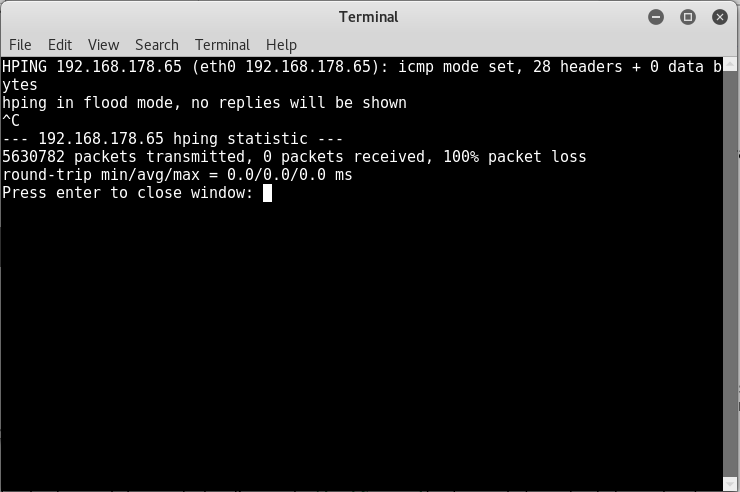
\includegraphics[width=\textwidth]{images/dos/pingflood}
	\caption{Stand des Tutorials nachdem der ARP-Scan durchfegührt wurde}
	\label{fig:pingflood}
\end{figure}

\subsection{SYN-Flooding} 

\subsubsection{Erklärung}

Die SYN-Flood Attacke verwendet das Grundprinzip des TCP Transportprotokolls um Dienste oder Server für den Nutzer unerreichbar zu machen. Normalerweise wird eine TCP Verbindung zwischen Client und Server auf Folgende Weise aufgebaut. 

\begin{itemize}
	\item Der Client fordert eine Verbindung mit dem Server an, indem er eine SYN(synchronize) Nachricht an den Server sendet.
	\item Der Server bestätigt die Anfrage indem er eine SYN-ACK(synchronize acknowledge) Nachricht an den Client zurückschickt. 
	\item Der Client antwortet nun mit einer ACK(acknowledge) Nachricht an den Server um den Verbindungsaufbau abzuschließen.
\end{itemize}
Dieser Vorgang wird der TCP Three-Way-Handshake genannt und ist die Grundlage für den verbindungsorientierten Aufbau mit dem TCP Protokoll.
	\begin{figure}[H]
		\centering
		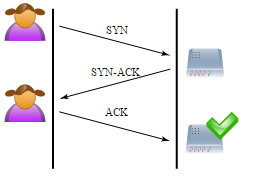
\includegraphics[width=0.9\textwidth]{images/dos/three_way_handshake.png}
		\caption{Normaler Ablauf beim TCP Verbindungsaufbau}
		\label{fig:three way handshake}
	\end{figure}

Die SYN-Flood Attacke funktioniert nun indem der Server nicht die von ihm erwartete ACK Nachricht erhält um die Verbindung vollständig aufzubauen.
Dies kann man dadurch realisieren, dass der Client keine ACK Nachricht an den Server zurückschickt. Eine der Möglichkeit ist das Spoofing der Client IP-Adresse. Dadurch sendet der Server die SYN-ACK Nachricht an die falsche IP-Adresse. Der Client der nun die Nachricht erhält, wird nun nicht mit der ACK Nachricht antworten, da er nie eine SYN Nachricht zum Verbindungsaufbau an diesen Server geschickt hat.

	\begin{figure}[H]
		\centering
		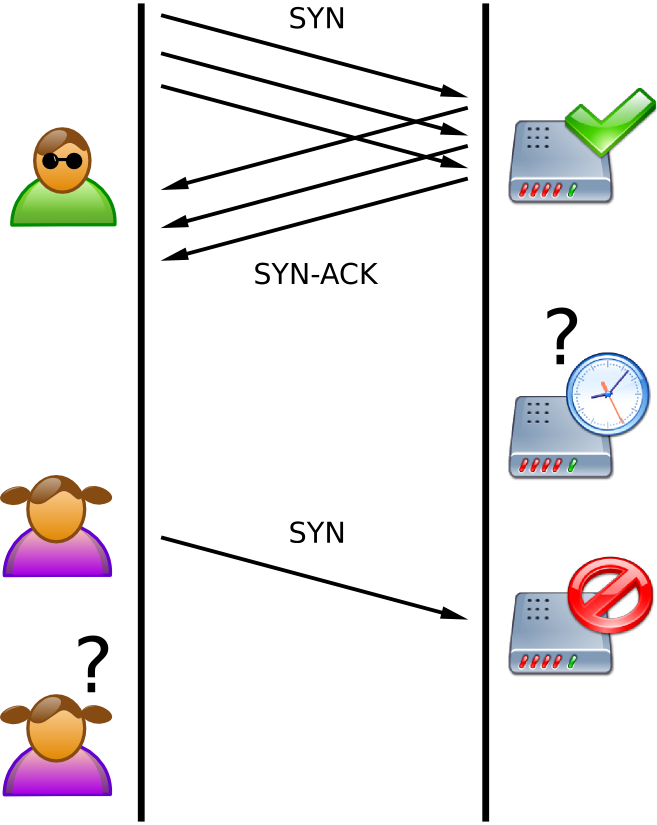
\includegraphics[width=0.9\textwidth]{images/dos/syn_flood_theorie.png}
		\caption{Kommunikationsablauf beim Syn Flood}
		\label{fig:syn flood theorie}
	\end{figure}
Der Server wartet eine gewisse Zeit auf die ACK Antwort des Clients, da durch den normalen Netzwerkverkehr auch Verzögerungen entstehen können. In dieser Zeit werden Ressourcen für diese so genannten "halb offenen Verbindungen" auf dem Server reserviert. Durch Flutung des Servers mit SYN Nachrichten wird nun versucht, die Ressourcen des Servers auzubrauchen. Sollten alle Ressourcen aufgebraucht sein, können keine weiteren Verbindungen mehr mit dem Server aufgebaut werden und es findet eine Dienstblockade statt.
In manchen Fällen kann es passieren, dass der angegriffene Server sogar abstürzt.

\subsubsection{Demonstration}

Zum Start der Demonstration muss zuerst auf dem SYN-Flood Opfer das OpferSynFlood Script ausgeführt werden.  

Zuerst wird ein Apache2 Webserver in einem Docker-Container gestartet gestartet.
\begin{lstlisting}
/etc/init.d/apache2 start
\end{lstlisting}
	\begin{figure}[H]
		\centering
		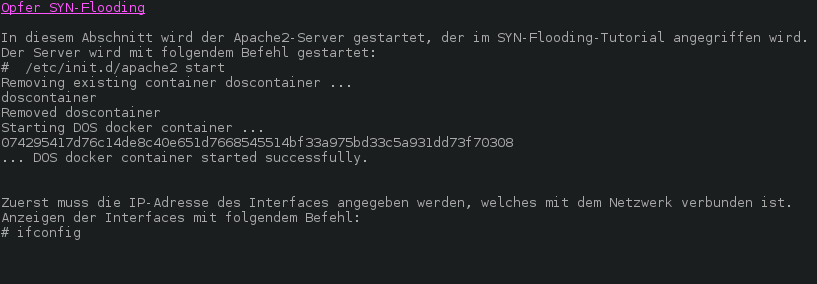
\includegraphics[width=\textwidth]{images/dos/dos_syn_opfer_server_start.png}
		\caption{Starten des Apache Servers}
		\label{fig:start opfer apache}
	\end{figure}

Im Anschluss werden die Netzwerkinterfaces angezeigt.
\begin{lstlisting}
ifconfig
\end{lstlisting}

Durch die Eingabe der eigenen IP-Adresse und der IP-Adresse des Angreifers wird nun der Filterstring erstellt, mit dem in Wireshark die Pakete die zwischen beiden IP-Adressen verschickt werden, angezeigt werden.

Zum Abschluss des Skripts wird der Docker-Container, in dem der Apache2 Server läuft, wieder gestoppt. Dies sollte nur geschehen, wenn der Angriff bereits ausgeführt wurde.
\begin{lstlisting}
/etc/init.d/apache2 stop
\end{lstlisting}

\newpage Im Angreifer Script  \colorbox{altgray}{\lstinline|SYNFLOOD|} werden zuerst alle Netzwerkinterfaces angezeigt.
\begin{lstlisting}
ifconfig
\end{lstlisting}
Die eigene IP Adresse muss nun im Hauptfenster eingegeben werden. 
Nun wird daraus ein IP Table Eintrag erstellt.
\begin{lstlisting}
iptables -A OUTPUT -p tcp -s Eigene IP_Adresse --tcp-flags RST RST -j DROP
\end{lstlisting}

\begin{itemize}
	\item \bashCommand{iptables} Definiert, dass nachfolgend in iptables eintrag folgt
	\item \bashCommand{-A} Es wird eine neue IP Tables Regel erstellt
	\item \bashCommand{OUTPUT} Die Regel wird auf Pakete angewandt, welche von einem lokalen Prozess stammen
	\item \bashCommand{-p tcp} Das Paket wird geprüft, wenn TCP das Verbindungsprotokoll ist
	\item \bashCommand{-s Eigene IP Adresse} Das Paket wird nur geprüft, wenn es von dieser IP Adresse stammt (In unserem Beispiel die eigene)
	\item \bashCommand{--tcp-flags RST RST} Die TCP Pakete mit dem RST Flag sind betroffen
	\item \bashCommand{-j DROP} Legt fest, dass Pakete gedropt werden sollen
\end{itemize}

Dieser Eintrag wird benötigt, da verhindert werden muss, dass dem Server nach der SYN-ACK Nachricht geantwortet werden soll. 

Anschließend wird Wireshark geöffnet, da dies später zur Veranschaulichung des Beispiels verwendet wird.
\begin{lstlisting}
wireshark &
\end{lstlisting}

Nach Eingabe der anzugreifenden IP-Adresse und des Ports an dem angegriffen werden soll, wird der Wireshark String erstellt.(Kopieren mit Strg + Shift + C)
	\begin{figure}[H]
		\centering
		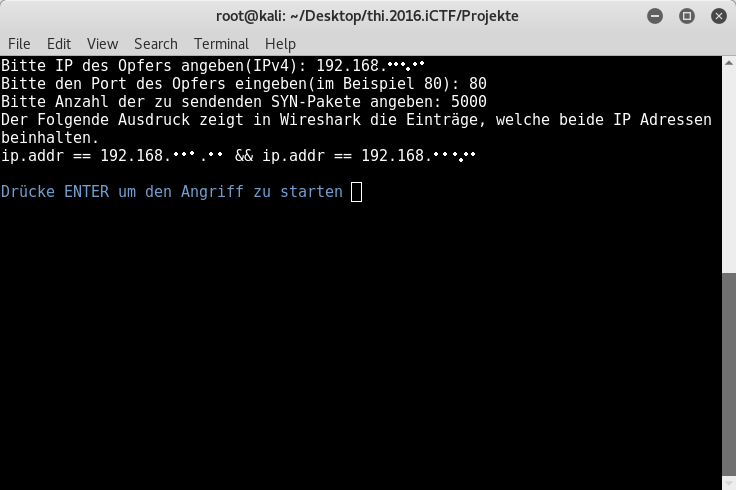
\includegraphics[width=0.9\textwidth]{images/dos/wireshark_string.png}
		\caption{Beispielstring für wireshark}
		\label{fig:wireshark string}
	\end{figure}
Nun sollte in Wireshark der entsprechende Netzwerkadapter ausgewählt werden. Der zuvor erstellte String wird nun oben in das Feld eingetragen. Dadurch werden nur noch Pakete angezeigt, die beide IP Adressen beinhalten.
Wird nun im Terminal die Attacke gestartet, so wird im selben Terminal bei jedem Angriff eine Nachricht mit ausgegeben.
	\begin{figure}[H]
		\centering
		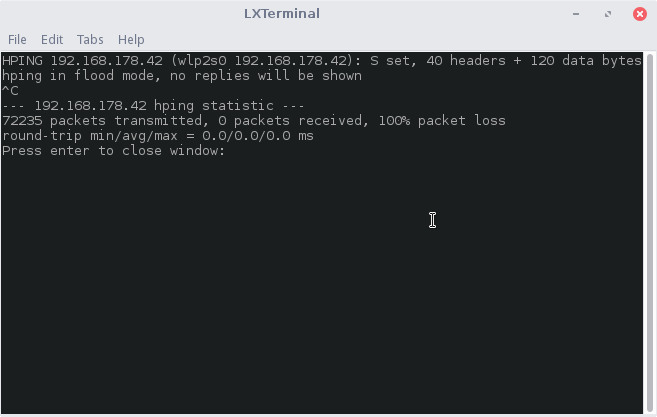
\includegraphics[width=0.9\textwidth]{images/dos/dos_syn_hping3_attack.png}
		\caption{Terminal beim SYN Flood Angriff}
		\label{fig:synattack example}
	\end{figure}
Nachdem die IP-Adresse und der Port des anzugreifenden Services eingegeben wurden, wird der Angriff durchgeführt.
Dem Benutzer wird daraufhin die Möglichkeit geboten durch Eingabe von Y oder y nochmals eine Attacke zu starten.
Wird nochmals eine Attacke gestartet, landet man direkt bei der Eingabe der Daten des Opfers. 


\subsection{Ping of Death}

Ein weiterer Dos Angriff ist der Ping of Death. Der Ping of Death ist ein älterer DoS Angriff der auf älteren Betriebssystemen möglich war. Dieses und die nächste Attacke wurden nur als Beispiel für ältere Attacken mit in die Dokumentation aufgenommen, da sie in jedem Fachbuch vorkommen und für das bessere Verständnis der DoS Attacken behilflich sind.

Die Grundlage für diesen Angriff ist die Spezifikation von ICMP-Echo Nachrichten, welche nur 2\^16 oder 65.536 Bytes im Datenabschnitt der Paketes enthalten  dürfen. Von älteren Betriebssystemen wurde dies öfter nicht beachtet, da die wichtigen Informationen für den Transfer im Header enthalten sind. Bei einigen dieser Betriebssysteme hat das überschreiten dieser Spezifikation zum Absturz geführt. Eine ICMP-Echo Nachricht dieser art wurde aus diesem grund Ping of Death genannt. 

\subsection{Teardrop}

Aus einem ähnlichen Grund wie zuvor beim Ping of Death ist der Teardrop Angriff entstanden. Beim Teardrop werden fragmentierte Pakete an das Opfer gesendet. Bei Fragmentierten Paketen werden die im Header gespeicherten Offsets genutzt um das ursprüngliche Paket ohne Überschneidungen wiederherzustellen. 
Um den Teardrop Angriff nun zu realisieren, werden Pakete mit sich überlagernden Offsets gesendet. Manche Betriebssysteme waren darauf nicht vorbereitet und stürzten ab. 
Betriebssysteme auf die dies zutraf, sind : Windows 3.1, Windows 95, Windows NT und Linux Kernels vor der Version 2.1.63. 

\section{Gegenmaßnahmen}

\begin{itemize}
	\item Intelligente Firewall einsetzen, die Angriffe automatisch erkennt und dynamisch Sperrlisten erzeugt und somit Pakete von bestimmten IP-Adressen (Angreifer) verwerfen oder umleiten
	\item Nutzung eines Filter-Services. Diese werden von mehreren kommerziellen Anbietern offeriert, die teilweise über Anbindungen von 400 bis 500 GBit/s verfügen. Selbst größte Angriffe können so ohne Störung des eigenen Rechenzentrums gefahrlos bewältigt werden. Die Dienste unterscheiden sich in Qualität und Größe der abfangbaren Angriffe. 
	\item In manchen Fällen kann es helfen sein Betriebssystem auf den neuesten Stand zu halten, da die Angreifer die Schwachstellen in veralteten Versionen ausnutzen.
	\item Syn Cookies können gegen das SYN-Flooding eingesetzt werden. Steigt die Anzahl der Verbindungsanfragen, so schickt der Server einfach die SYN-ACK Antwort zurück, löscht aber die SYN Anfrage. Sollte eine ACK Nachricht zurück an den Server kommen, so kann der Server die ursprünglich gestellte SYN Anfrage mit Hilfe von kodierten Informationen in der TCP Sequenznummer wiederherstellen.  
\end{itemize}




